\documentclass[11pt,a4paper]{article}
\usepackage[margin=2.5cm]{geometry}
\usepackage{graphicx}
\usepackage{hyperref}
\usepackage{booktabs}
\usepackage{amsmath}

\title{\textbf{Polar Sea-Ice Timing: Classical Trends and a Rigorous Spatial Null Test}\\[0.4em]
\large University of Hamburg --- M.Sc. Data Science \& AI (6-credit sea ice course, June/July 2026)}
\author{Omkar Kondhalkar}
\date{}

\begin{document}
\maketitle

\begin{abstract}
We analyse whether polar sea-ice \emph{timing} has shifted over the satellite era. Phase~1 (submitted one-pager) finds no statistically significant trend in Arctic minimum day-of-year (DOY; $-0.08$~d~yr$^{-1}$, $p=0.65$) or Antarctic AFIN breakup proxy ($+29.45$~d~yr$^{-1}$, $p=0.21$). Phase~2 tests a natural follow-up hypothesis: does pre-melt (July) sea-ice concentration (SIC) spatially predict which years have an early vs.\ late minimum? Using NSIDC CDRv6 G02202 (1979--2025, $n=45$ years with valid Phase~1 labels), we compute a pixel-wise Pearson correlation map and an early/late tercile composite, then test both for statistical robustness. \textbf{After Benjamini--Hochberg false-discovery-rate (FDR) correction across 15{,}883 ocean grid cells, zero pixels remain significant at $q=0.05$}, and region-averaged tests for the Beaufort Sea, Kara Sea, and marginal ice zone (MIZ) are individually non-significant ($p=0.96$, $0.45$, $0.39$). \textbf{Magnitude loss $\neq$ calendar shift, and naive pre-melt SIC does not explain interannual timing variability either} --- both the temporal and the spatial hypotheses point to the same conclusion: minimum-timing variability behaves as internal noise at the pixel level, not a fixed, learnable geographic fingerprint.
\end{abstract}

\section{Introduction}
Sea-ice \emph{timing}---when ice reaches its annual minimum (Arctic) or when coastal fast ice breaks up (Antarctica)---controls melt-season length. An earlier Arctic minimum strengthens ice--albedo feedback (Notz \& Stroeve, 2016). At Neumayer Station~III, the Alfred Wegener Institute operates the AFIN fast-ice program in Atka Bay. Phase~1 asks whether minimum \emph{timing} has shifted; Phase~2 asks \emph{why} interannual variability exists when the scalar trend is non-significant, and specifically tests whether pre-melt spatial SIC structure predicts it.

\section{Methods}

\subsection{Phase 1 (unchanged)}
\textbf{Arctic:} OSI SAF daily hemispheric SIA; annual minimum DOY in July--December, 1979--2025. OLS trend, 95\% bootstrap CI (5000 resamples).

\textbf{Antarctic:} AFIN manual transect surveys (PANGAEA 2010--2018, $n=9$). Breakup proxy = last survey date per season (Arndt et al., 2020).

\subsection{Phase 2: spatial null test}
\textbf{Sensitivity (Figs.~2--3).} Dual-axis plot of SIA at minimum vs.\ minimum DOY; Aug~31 hemispheric SIA vs.\ minimum DOY scatter (scalar baseline context).

\textbf{Spatial Pearson-$r$ + composite (Fig.~5).} NSIDC CDRv6 G02202 monthly SIC (25~km polar stereographic, 60--90$^\circ$N cap, 160$\times$160 pixels, $n=45$ years with a valid Phase~1 minimum-DOY label). Years ranked by observed minimum DOY into early/late terciles ($n=15$ each). For every grid cell: Pearson $r$ and two-sided $t$-test $p$-value between July SIC (1979--2025) and annual minimum DOY. Composite map: mean July SIC (early tercile) $-$ mean July SIC (late tercile). Sea-ice edge contour at 15\% SIC; Beaufort, Kara, and MIZ sub-regions annotated per Nie et al.\ (2025) and Yang et al.\ (2024).

\textbf{Multiple-comparison correction.} With 15{,}883 ocean grid cells tested independently, $\sim$794 would appear ``significant'' at $\alpha=0.05$ by chance alone. We therefore apply Benjamini--Hochberg FDR correction ($q=0.05$) across all ocean cells, and separately compute a single region-averaged time series (SIC spatially averaged over each named box, then correlated with DOY) for Beaufort, Kara, and MIZ --- a 3-hypothesis test immune to the pixel-multiplicity problem.

\textbf{CMIP6 (literature only).} We cite Gregory et al.\ (2024, \textit{GRL}) and Frankignoul et al.\ (2024, \textit{J.~Climate}) for CMIP6 September SIC biases. Models with significant timing trends where observations lack them may overestimate forced timing shifts; we do not recompute CMIP6 timing here.

\section{Results}

\begin{figure}[ht]
  \centering
  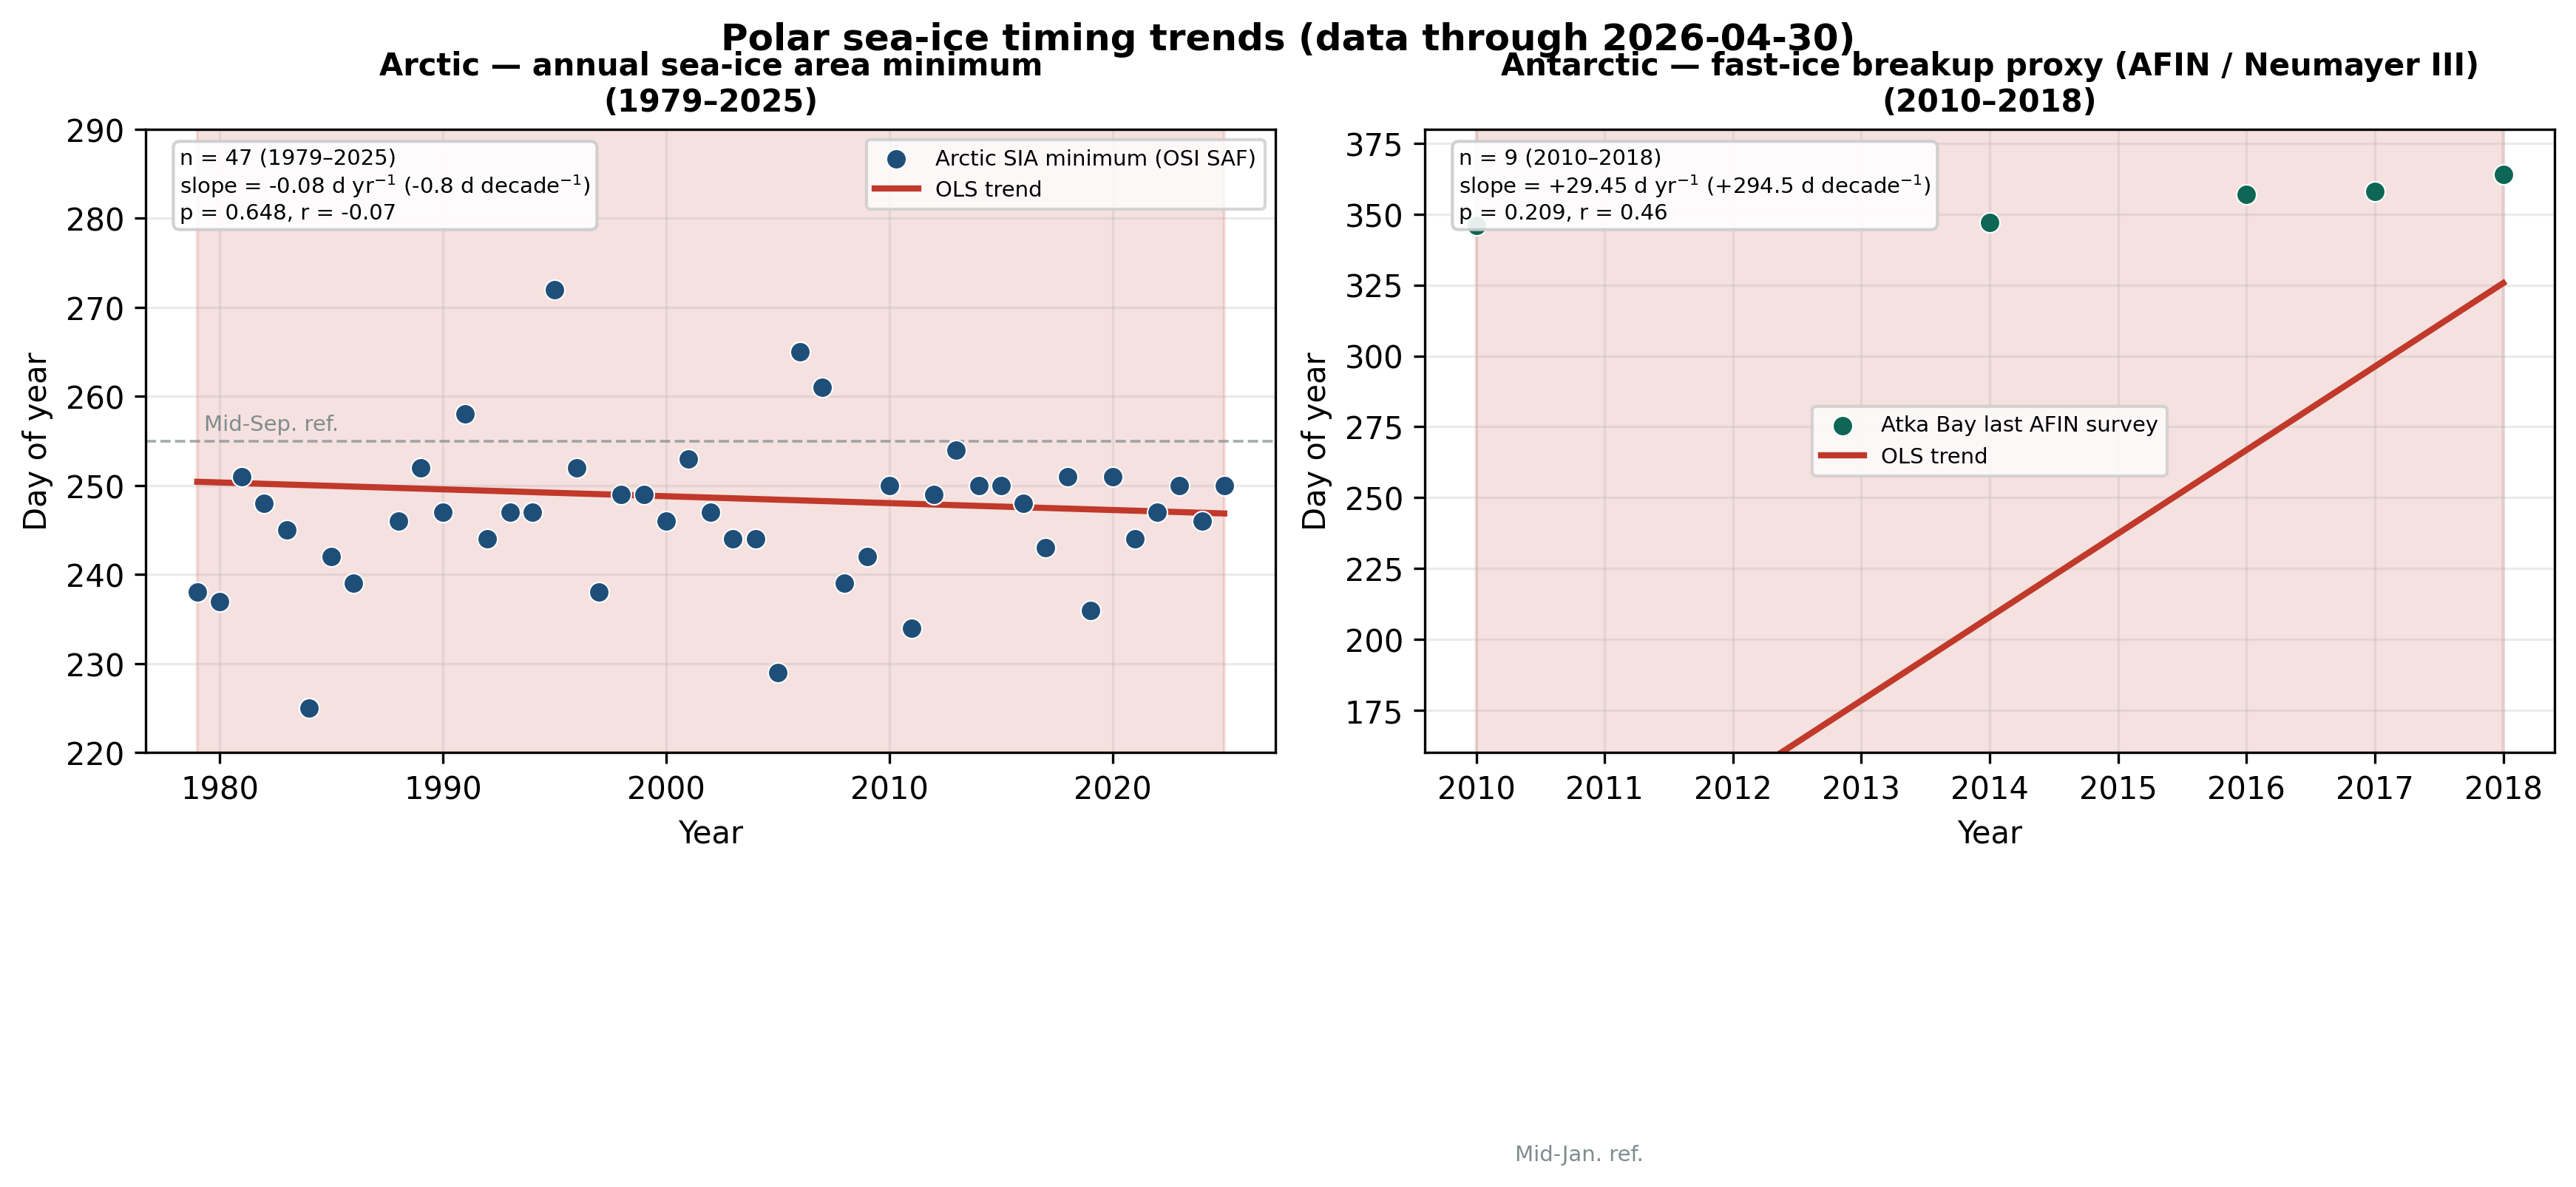
\includegraphics[width=\linewidth]{../results/figures/polar_ice_timing_comparison.png}
  \caption{Phase~1: Arctic SIA minimum DOY (left) and Antarctic AFIN breakup proxy (right). No significant timing trends.}
\end{figure}

\begin{figure}[ht]
  \centering
  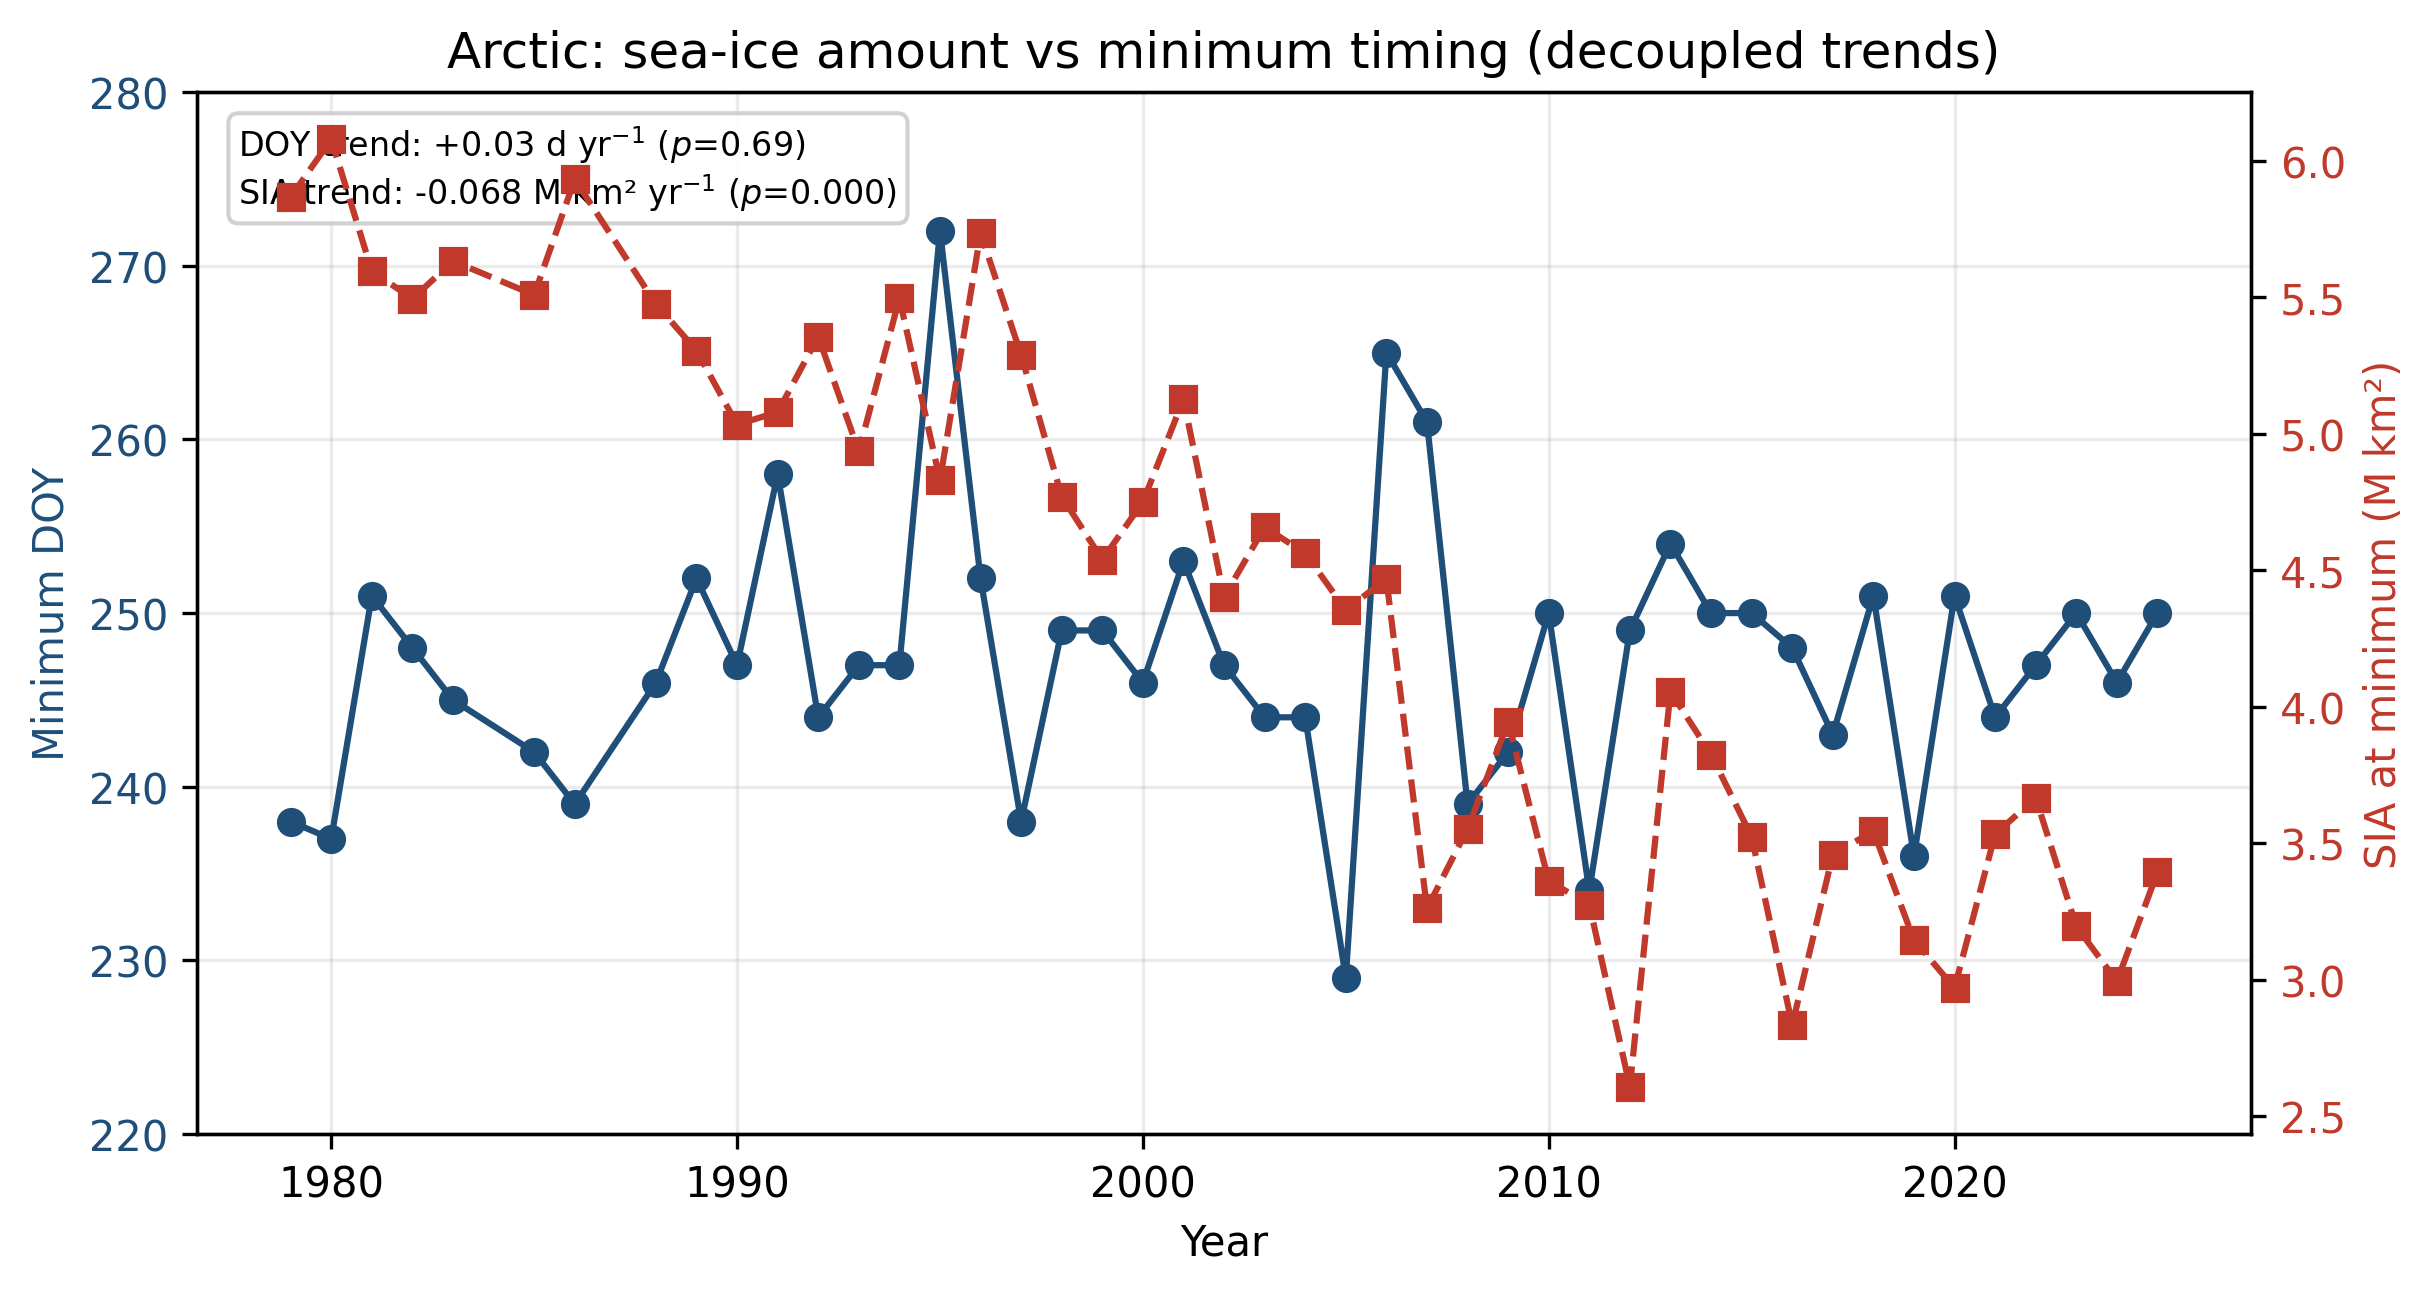
\includegraphics[width=\linewidth]{../results/figures/arctic_sia_minimum_vs_doy_dual_axis.png}
  \caption{Arctic SIA at minimum (red) declines while minimum DOY (blue) shows no robust trend---visual decoupling of magnitude and timing.}
\end{figure}

\begin{figure}[ht]
  \centering
  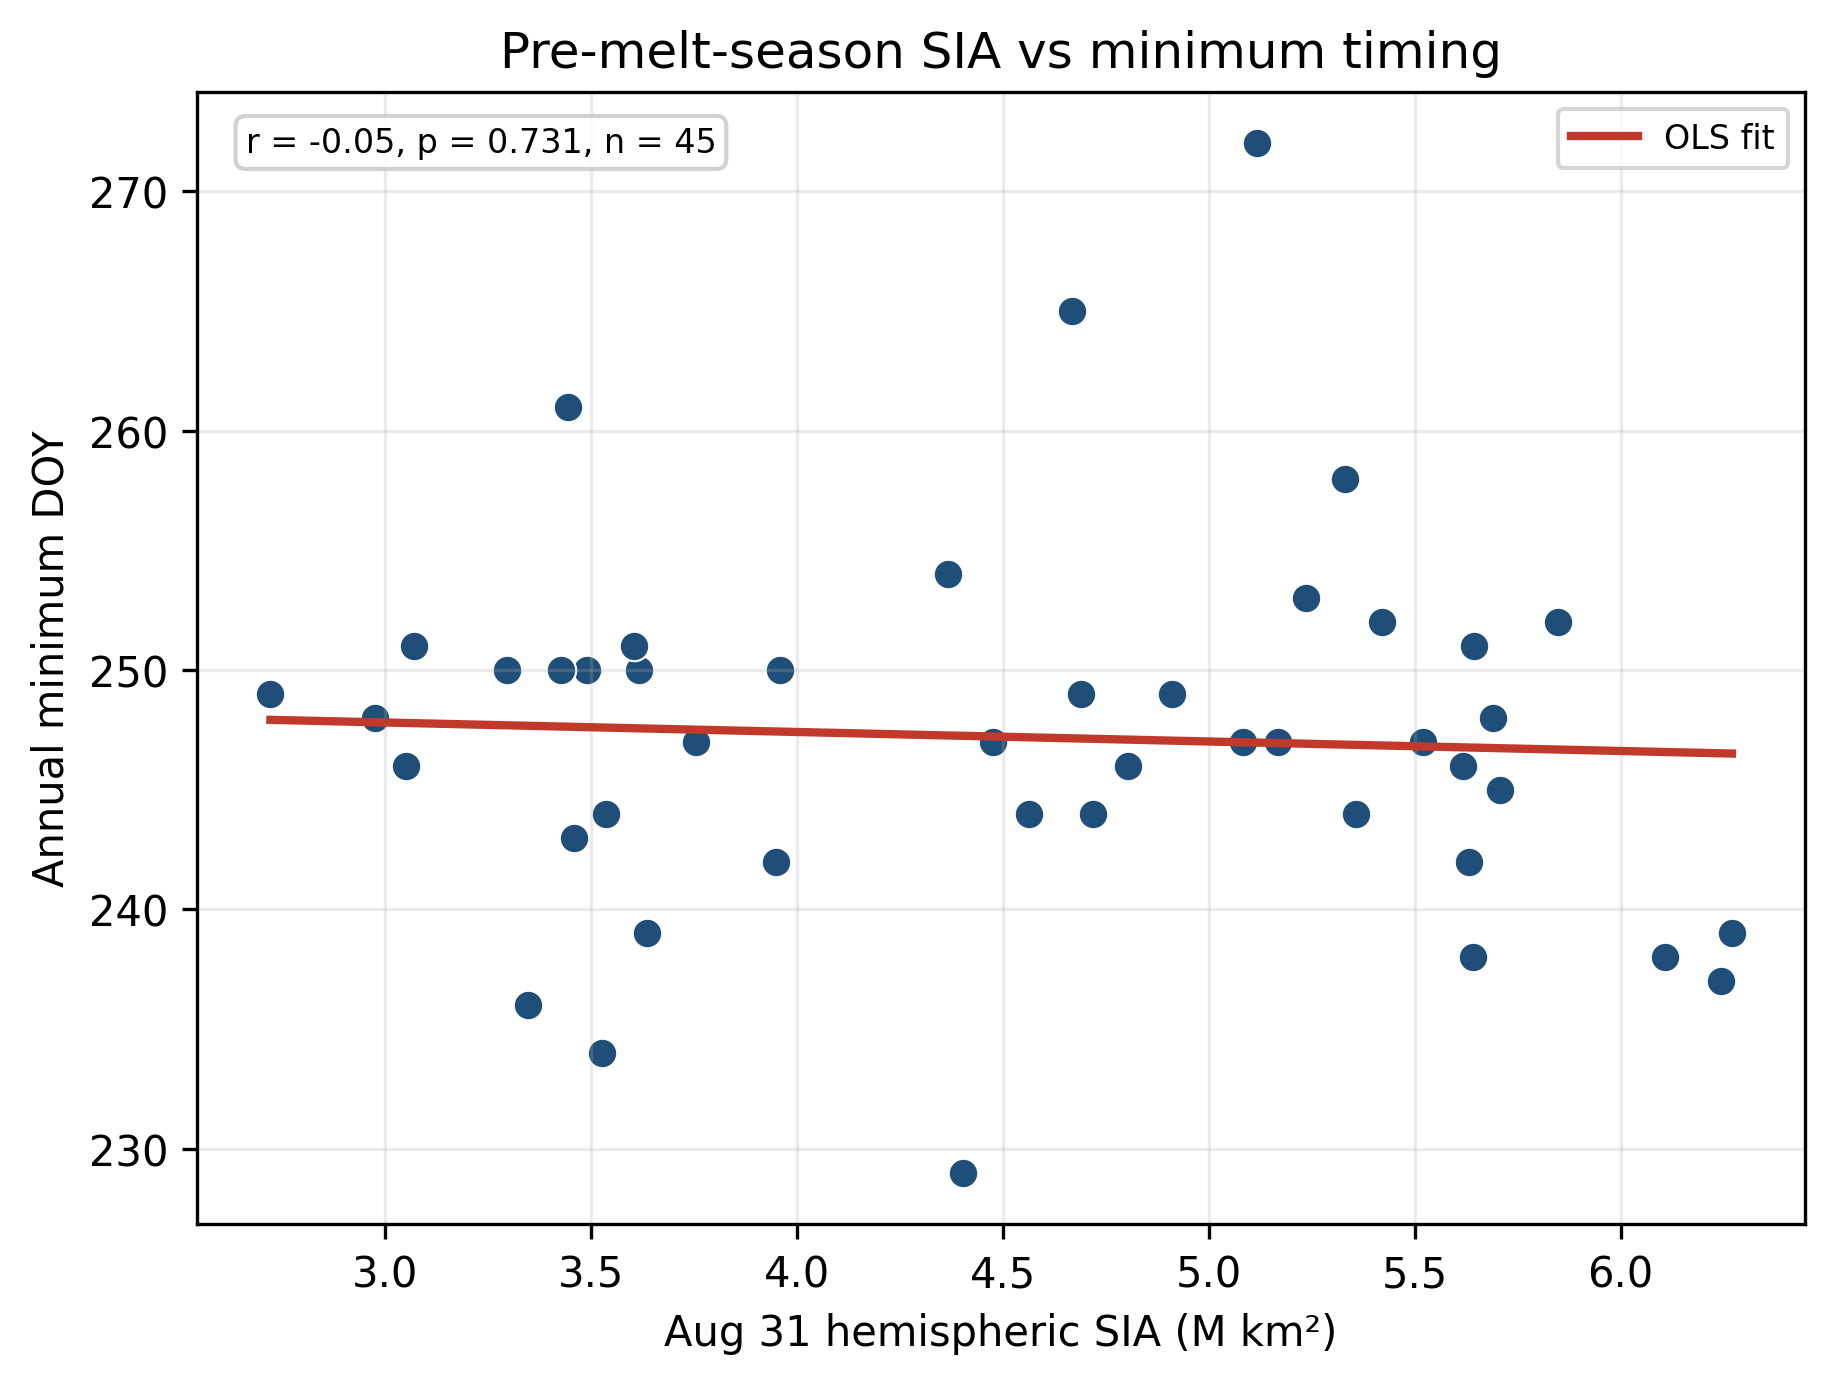
\includegraphics[width=0.72\linewidth]{../results/figures/arctic_aug31_sia_vs_min_doy.png}
  \caption{Aug~31 hemispheric SIA vs.\ annual minimum DOY (scalar mechanistic context).}
\end{figure}

\begin{figure}[ht]
  \centering
  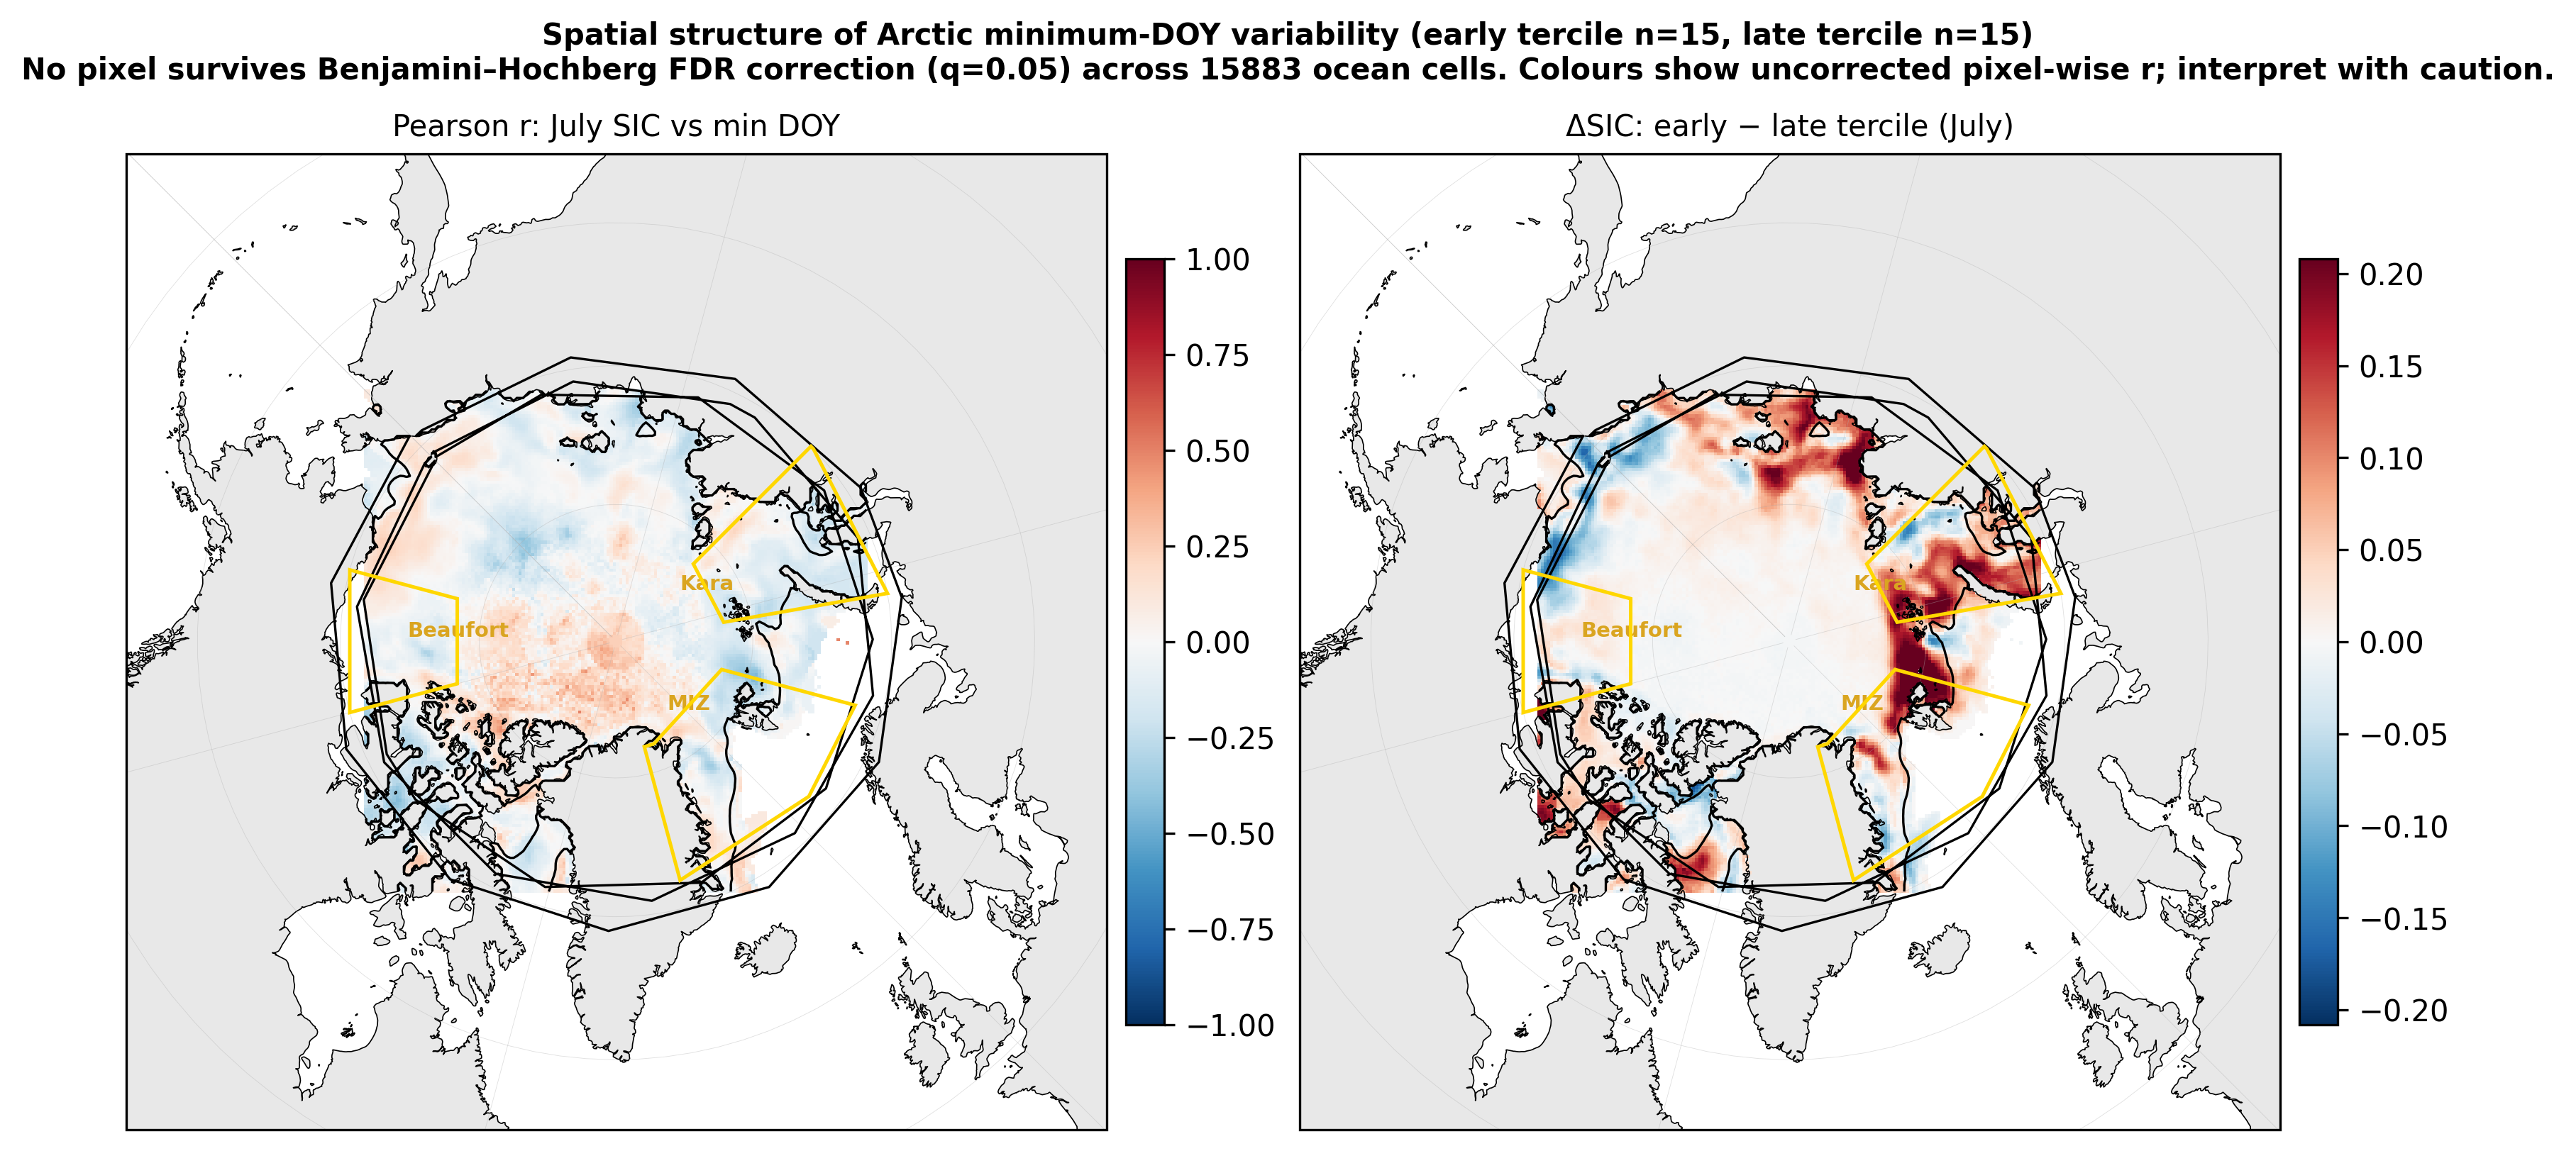
\includegraphics[width=\linewidth]{../results/figures/fig5_spatial_heatmap.png}
  \caption{Left: pixel-wise Pearson $r$ between July SIC and minimum DOY (uncorrected). Right: early-minus-late tercile July SIC composite. \textbf{No pixel survives FDR correction} ($q=0.05$) across 15{,}883 ocean cells; the visually plausible ``hot spots'' are consistent with the $\sim$442 cells expected from multiple testing (below the $\sim$794 expected by chance, i.e.\ fewer nominal hits than pure noise would produce). Region-averaged tests are likewise non-significant: Beaufort $r=0.01$, $p=0.96$; Kara $r=-0.11$, $p=0.45$; MIZ $r=-0.13$, $p=0.39$ ($n=45$).}
\end{figure}

\begin{figure}[ht]
  \centering
  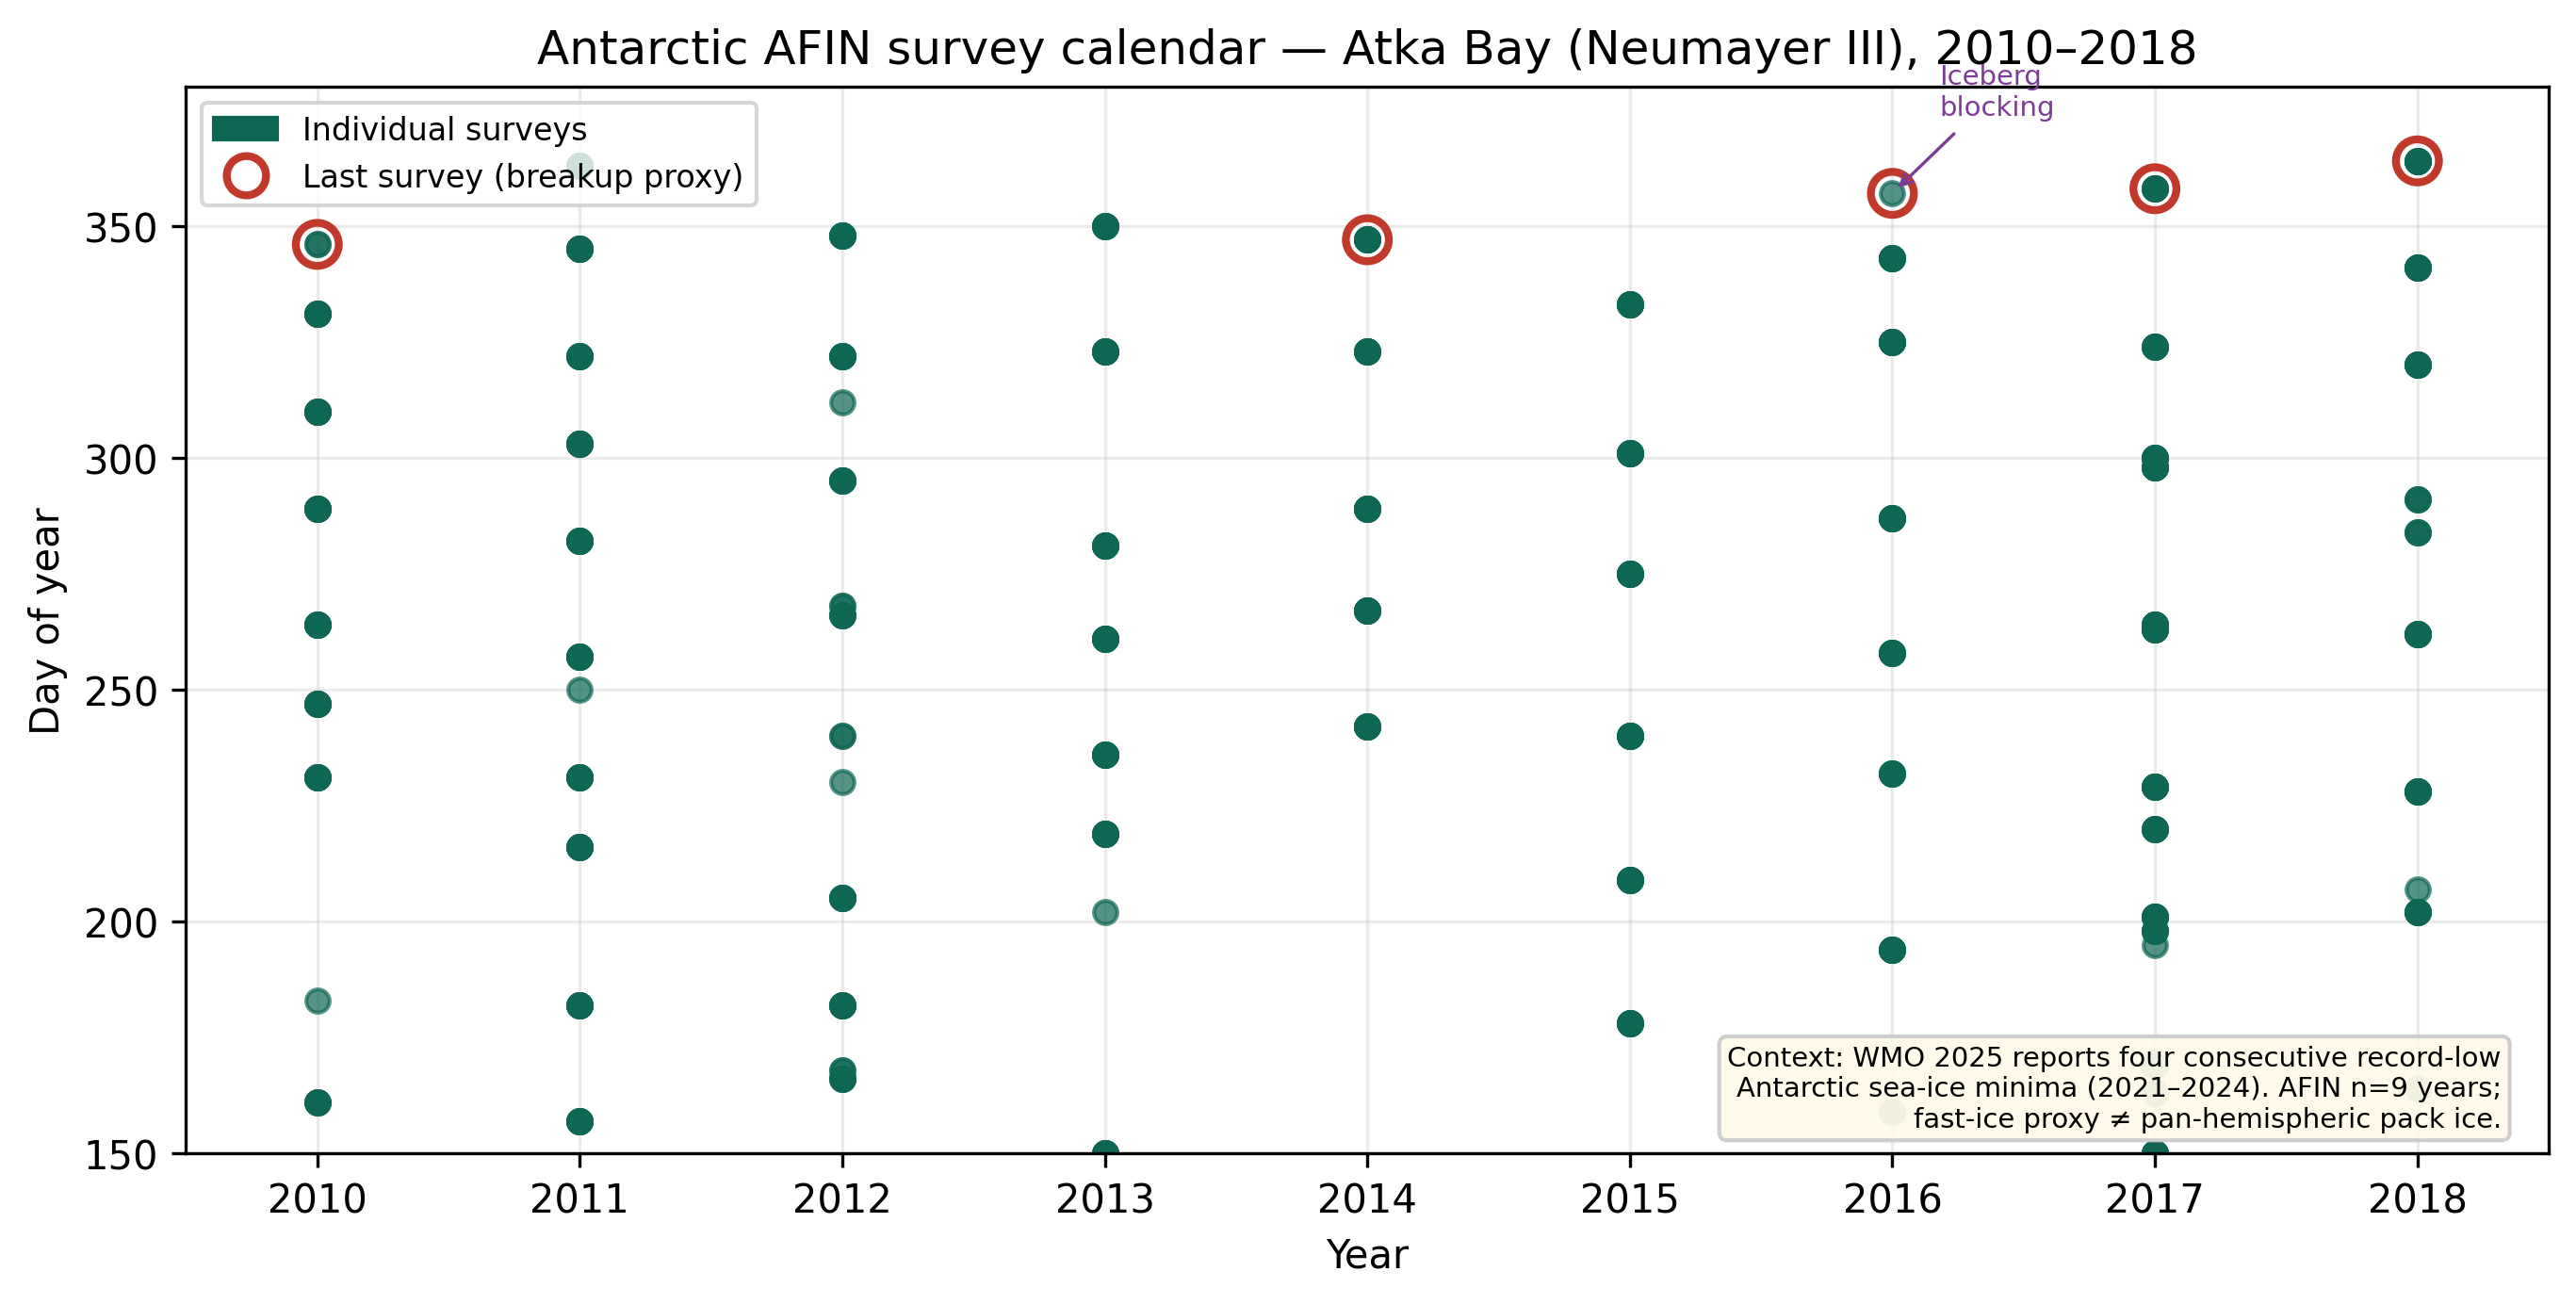
\includegraphics[width=\linewidth]{../results/figures/antarctic_afin_calendar.png}
  \caption{Antarctic AFIN survey calendar with 2013/2016 iceberg-blocking annotations and WMO~(2026) context (four lowest Antarctic sea-ice minima on record, 2022--2025).}
\end{figure}

\section{Discussion}
Pan-hemispheric sea-ice minimum timing shows no statistically significant trend in either hemisphere (Phase~1). Phase~2 tested the natural follow-up hypothesis that pre-melt (July) SIC spatially preconditions which years are early vs.\ late. It does not, once tested rigorously: zero grid cells survive FDR correction, and none of the three literature-motivated regions (Beaufort, Kara, MIZ) shows an individually significant correlation. This null result is itself informative --- an uncorrected pixel map with $\sim$15{,}900 independent tests will always show visually convincing ``hot spots'' by construction (apophenia), and reporting them without correction would be a textbook multiple-comparisons error.

This does not mean regional atmospheric forcing is irrelevant to timing --- it means \emph{static pre-melt ice state} is not the right predictor. Recent literature attributes Beaufort and Kara Sea ice-timing variability to \emph{synoptic-scale wind forcing during the melt season itself}: transient easterly wind events and Beaufort High repositioning drive the timing of ice export and opening in the Beaufort Sea (Nie et al., 2025, \textit{Remote Sensing}), while wind-driven ice transport similarly governs open-water onset timing in the Kara Sea (Yang et al., 2024, \textit{J.~Climate}). Separately, Wang et al.\ (2026, \textit{GRL}) show that short-term (daily) SIC variability in the Arctic MIZ has risen 11.4\% since 2007 via an air--sea heat-flux feedback --- evidence that the MIZ is dynamically noisy in general, consistent with (rather than contradicting) our finding that a single static July snapshot cannot predict the September minimum date there.

The Antarctic analysis remains limited to $n=9$ years (2010--2018) of AFIN manual transect proxy data at Atka Bay. OSI-SAF Southern Hemisphere minimum DOY is used only for contextual annotation.

\section{Conclusion}
\textbf{Magnitude loss $\neq$ calendar shift --- and naive spatial preconditioning does not explain the noise either.} Phase~1 establishes non-significant scalar timing trends in both hemispheres. Phase~2 tested whether spatial SIC structure explains the variability the scalar trend leaves unexplained; after correcting for the number of grid cells tested, it does not. Timing variability is best explained not by antecedent ice state but by within-season atmospheric circulation (Beaufort High strength, easterly wind bursts) documented in recent literature --- a concrete, testable direction for future work (e.g.\ correlating minimum DOY with ERA5 wind fields) that lies beyond this course's scope.

\small
\textbf{Data:} OSI SAF; NSIDC CDRv6 G02202; PANGAEA AFIN; Arndt et al.\ (2020).\\
\textbf{Cited literature:} Gregory et al.\ (2024, \textit{GRL}); Frankignoul et al.\ (2024, \textit{J.~Climate}); Nie, Zheng, Wei, Zhao \& Luo (2025, \textit{Remote Sensing}, 17(19), 3286); Yang, Nie, Zhang, Luo, Wei \& Zhao (2024, \textit{J.~Climate}, 37(4), 1367--1381); Wang, Lohmann, Gou et al.\ (2026, \textit{Geophysical Research Letters}, 53(7), doi:10.1029/2025GL119415); WMO (2026), \textit{State of the Global Climate 2025}.

\end{document}
